%iffalse
\let\negmedspace\undefined
\let\negthickspace\undefined
\documentclass[journal,12pt,onecolumn]{IEEEtran}
\usepackage{cite}
\usepackage{amsmath,amssymb,amsfonts,amsthm}
\usepackage{algorithmic}
\usepackage{graphicx}
\usepackage{textcomp}
\usepackage{xcolor}
\usepackage{txfonts}
\usepackage{listings}
\usepackage{enumitem}
\usepackage{mathtools}
\usepackage{gensymb}
\usepackage{comment}
\usepackage[breaklinks=true]{hyperref}
\usepackage{tkz-euclide} 
\usepackage{listings}
\usepackage{gvv}                                        
%\def\inputGnumericTable{}                                 
\usepackage[latin1]{inputenc}                                
\usepackage{color}                                            
\usepackage{array}                                            
\usepackage{longtable}                                       
\usepackage{calc}                                             
\usepackage{multirow}                                         
\usepackage{hhline}                                           
\usepackage{ifthen}                                           
\usepackage{lscape}
\usepackage{tabularx}
\usepackage{array}
\usepackage{float}

\usepackage{enumitem}
\usepackage{xcolor}
%\usepackage{multicol}


\newtheorem{theorem}{Theorem}[section]
\newtheorem{problem}{Problem}
\newtheorem{proposition}{Proposition}[section]
\newtheorem{lemma}{Lemma}[section]
\newtheorem{corollary}[theorem]{Corollary}
\newtheorem{example}{Example}[section]
\newtheorem{definition}[problem]{Definition}
\newcommand{\BEQA}{\begin{eqnarray}}
\newcommand{\EEQA}{\end{eqnarray}}
\newcommand{\define}{\stackrel{\triangle}{=}}
\theoremstyle{remark}
\newtheorem{rem}{Remark}

\title{Vector Arithmetic (Section Formula)}
\author{AI24BTECH11021 - Manvik Muthyapu}
\begin{document}
\bibliographystyle{IEEEtran}

\maketitle
\bigskip

\renewcommand{\thefigure}{\theenumi}
\renewcommand{\thetable}{\theenumi}


\textbf{Question}:\\

Show that the points $\textbf{A}\brak{-6,10},\textbf{B}\brak{-4,6}$ and $\textbf{C}\brak{3,-8}$ are collinear and prove that $AB = \frac{2}{9}AC$.\\
		
\solution 

If the determinant 
$
\myvec{
1 & 1 & 1 \\
A & B & C}
$
is zero, then $A$, $B$, and $C$ are collinear.

\begin{align}
	\text{Det} =&
	\mydet{
1 & 1 & 1 \\
-6 & -4 & 3 \\
10 & 6 & -8
	} \\
&= 1 \cdot (32 - 18) - 1 \cdot (48 - 30) + 1 \cdot (-36 + 40) \\
&= 0
\end{align}

$\therefore$ $A$, $B$, and $C$ are collinear.\\

Using the section formula, if $B$ divides $AC$ in the ratio $m:n$, then:

\begin{align}
\brak{\frac{m \cdot 3 + n \cdot (-6)}{m+n}, \frac{m \cdot (-8) + n \cdot 10}{m+n}} &= (-4, 6) 
\end{align}

Equating the coordinates, we get
\begin{align}
\frac{m}{n} &= \frac{2}{7}
\end{align}

$\therefore$ It confirms that $B$ divides $AC$ in the ratio $2:7$. Since $B$ divides $AC$ in the ratio $2:7$, we have:

\begin{align}
\frac{AB}{AC} &= \frac{2}{2+7} = \frac{2}{9}
\end{align}

$\therefore AB = \frac{2}{9} AC$, Hence proved.

\begin{figure}[h!]
	\centering
	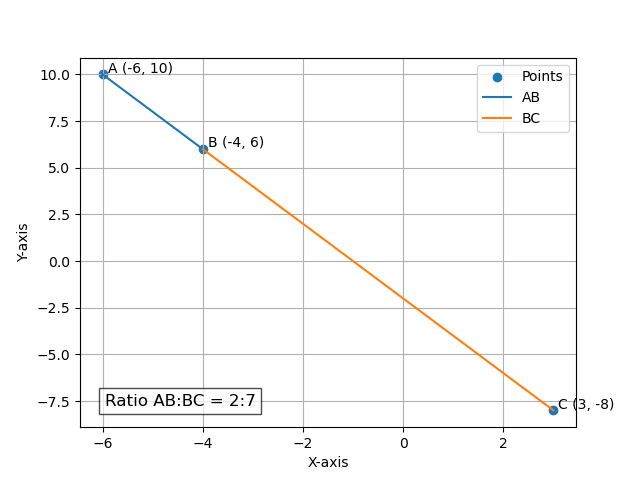
\includegraphics[width=0.7\linewidth]{figs/fig1.png}
\end{figure}
\end{document} 

